\documentclass{article}
\usepackage{fontspec}
\usepackage{amsmath}
\usepackage{marvosym}
\usepackage{graphicx}
\usepackage{fullpage}
\setmainfont{DejaVu Serif}

\begin{document}
\thispagestyle{empty}
\textbf{PHYS 211 --- Team Problem 11}
\hrule
\vspace{.3in}

Consider the following configuration of springs with two different spring constants, $k_1$, and $k_2$ and a block with mass $m$. Find the angular frequency of oscillation
for each situation. The block slides on a frictionless horizontal surface. Neglect the weights of the springs and any torques applied to the block.

Hint: Use hook's law and appropriate free-body diagrams to find the effective spring constant for each situtation and then use $\omega=\sqrt{\frac{k_{\text{eff}}}{m}}$

\begin{figure}[!ht]
  \centering
  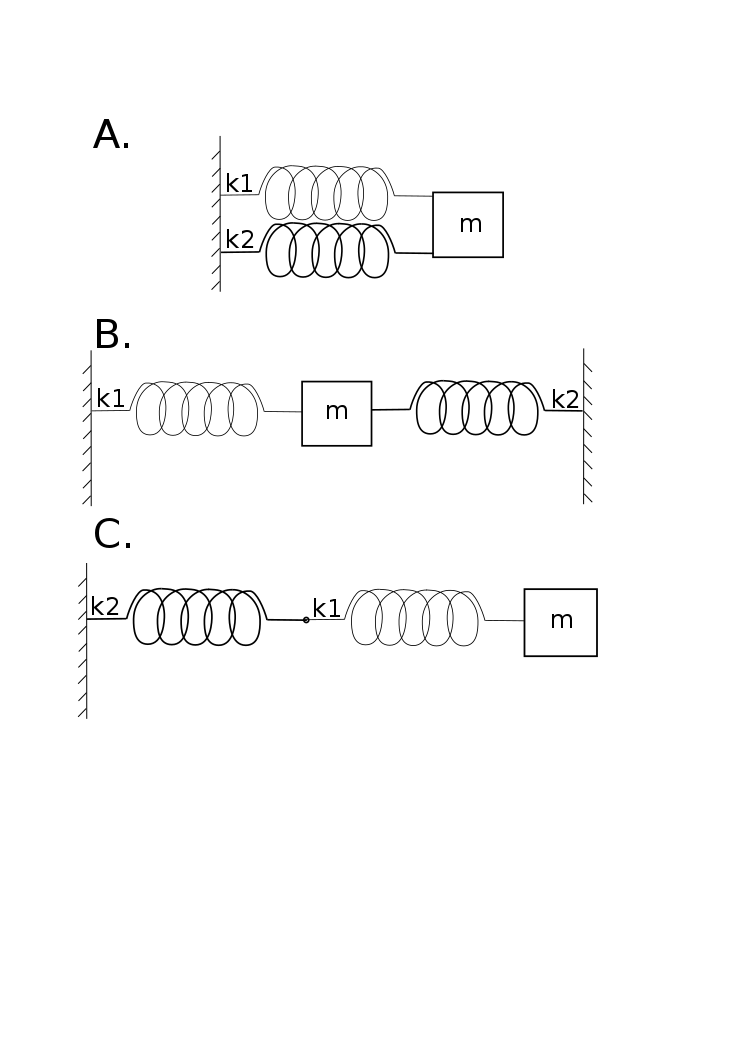
\includegraphics[height=0.7\textheight]{figures/springs}
\end{figure}


\end{document}
